%
%
%   LQuiz 13 : 2022--03--24 (R)
%
%

\section{Exercise}

% Reference : SHW
% Graphing tool : https://www.desmos.com/calculator

(4 pt) Let $f : \reals \rightarrow \reals$ be the piecewise function whose rule of assignment is
\begin{align*}
f(x)
=
\begin{dcases*}
-4		&	if $x \leq -1$		\\
2 x - 2	&	if $-1 \leq x \leq 2$	\\
x		&	if $x \geq 2$
\end{dcases*}
\end{align*}
The function $f$ is graphed below. This exercise explores the signed area under the graph of $f$ from $x = -3$ to $x = 4$.
\begin{center}
%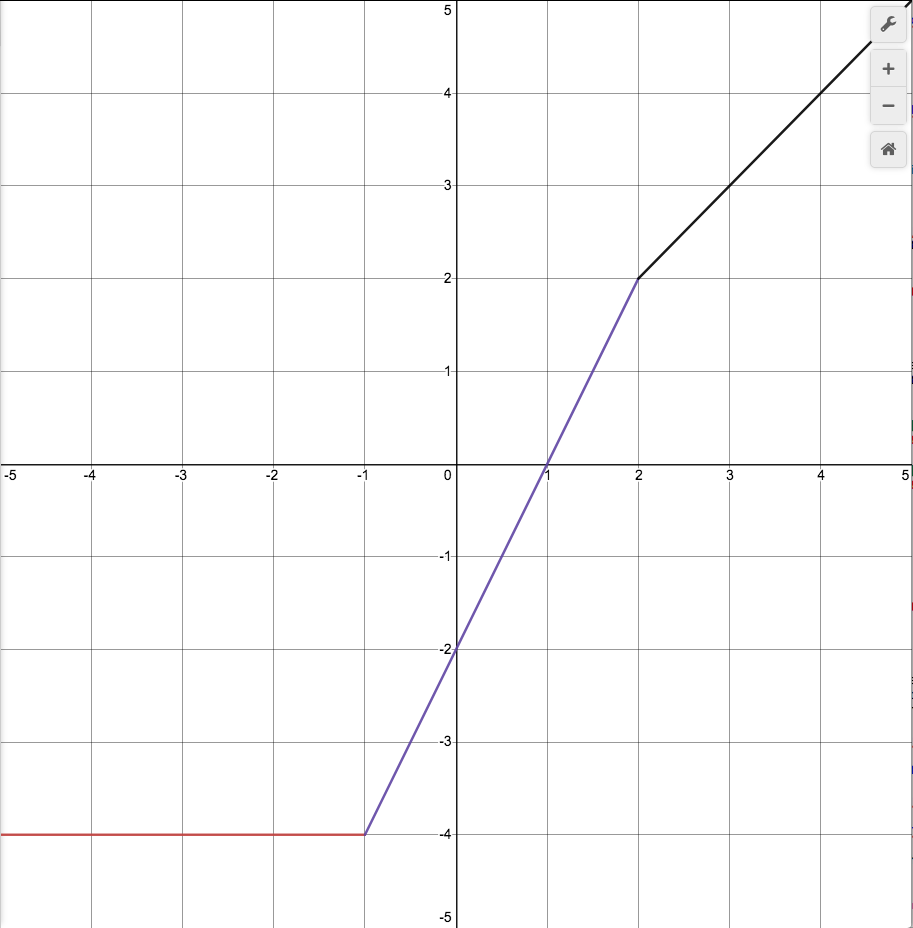
\includegraphics[width=0.2\textwidth]{\filePathGraphics/LQ13_Graph.png}% Activate for quiz.
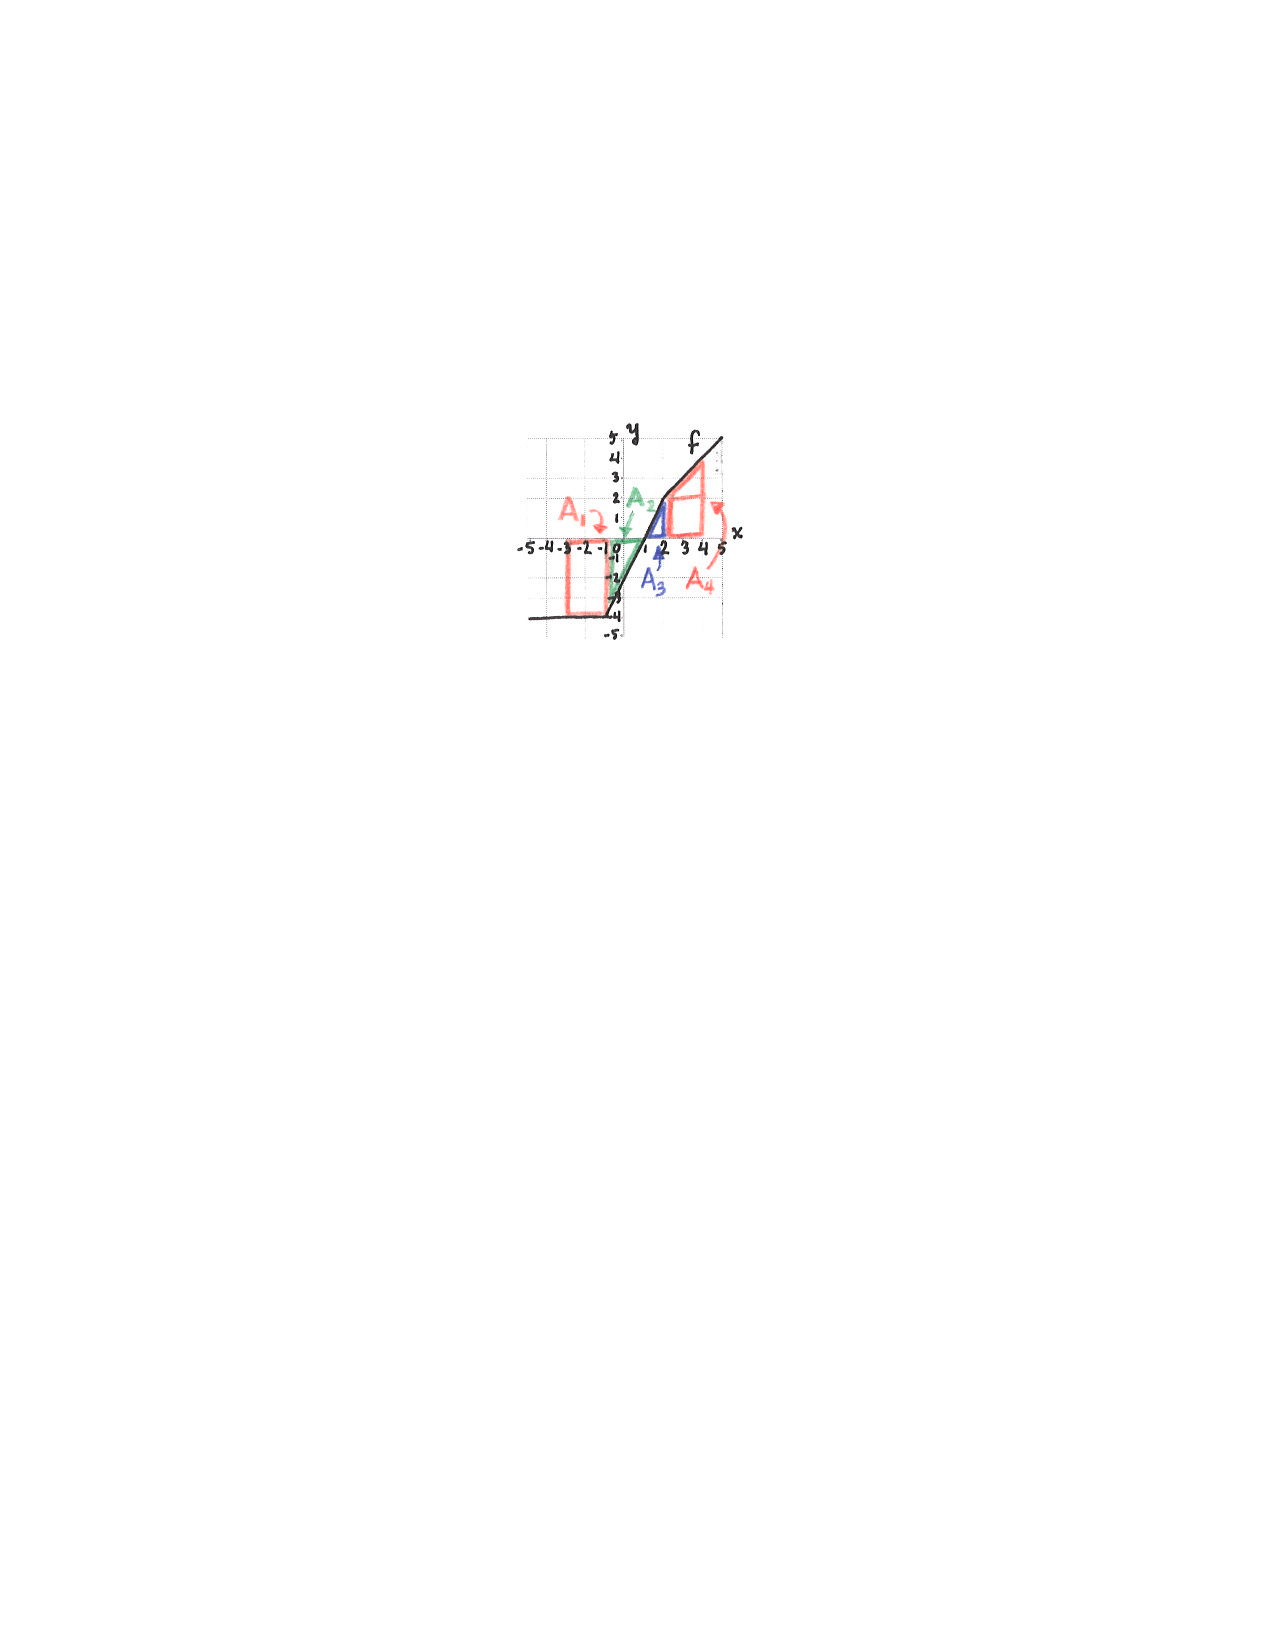
\includegraphics[scale=0.8]{\filePathGraphics/LQ13_Graph_Geometry.pdf}% Activate for solutions.
\end{center}



\begin{enumerate}[label=(\alph*)]
\item\label{itm : LQ13a} (1 pt) Use geometry to show that $\int_{-3}^{4} f(x) \spaceIntd \intd x = -5$.
\end{enumerate}

\spaceSolution{1in}{% Begin solution.
Partition the area between the graph of $f$ and the $x$-axis as shown above. We compute the signed area $A_{i}$ of each piece:% Begin footnote.
\footnote{Recall that the area is positive if it lies above the $x$-axis (corresponding to positive $y$-values), and negative if it lies below the $x$-axis (corresponding to negative $y$-values).}% End footnote.
\begin{align*}
A_{1}
&=
-(2) (4)
=
-8
&
A_{3}
&=
+\frac{1}{2} (1) (2)
=
1
\\
A_{2}
&=
-\frac{1}{2} (2) (4)
=
-4
&
A_{4}
&=
+\left[(2) (2) + \frac{1}{2} (2) (2)\right]
=
6
\end{align*}
Thus the total area is
\begin{align*}
A
=
A_{1} + A_{2} + A_{3} + A_{4}
=
-8 + (-4) + 1 + 6
=
-5
\end{align*}}% End solution.



\begin{enumerate}[resume,label=(\alph*)]
\item\label{itm : LQ13b} (2 pt) On separate graphs below, draw a lower sum and an upper sum, each with seven intervals of width $1$, to estimate $\int_{-3}^{4} f(x) \spaceIntd \intd x$. Show that $L \leq \int_{-3}^{4} f(x) \spaceIntd \intd x \leq U$.
\begin{center}
%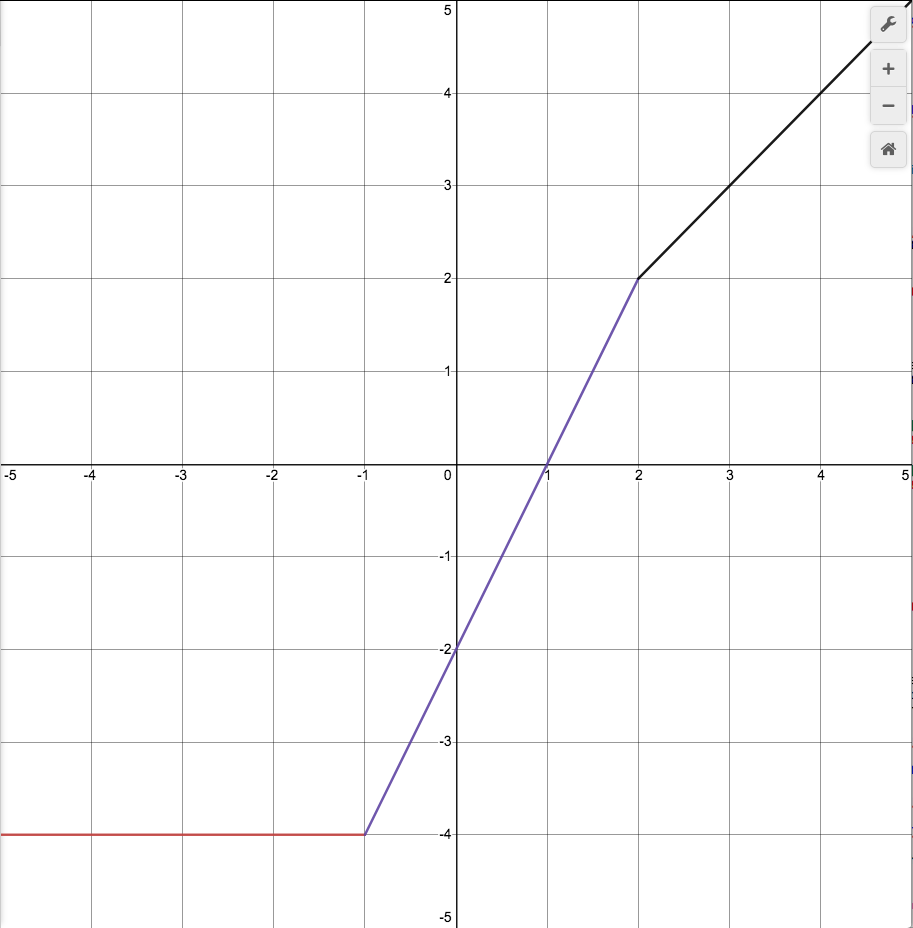
\includegraphics[scale=0.18]{\filePathGraphics/LQ13_Graph.png}% Activate for quiz.
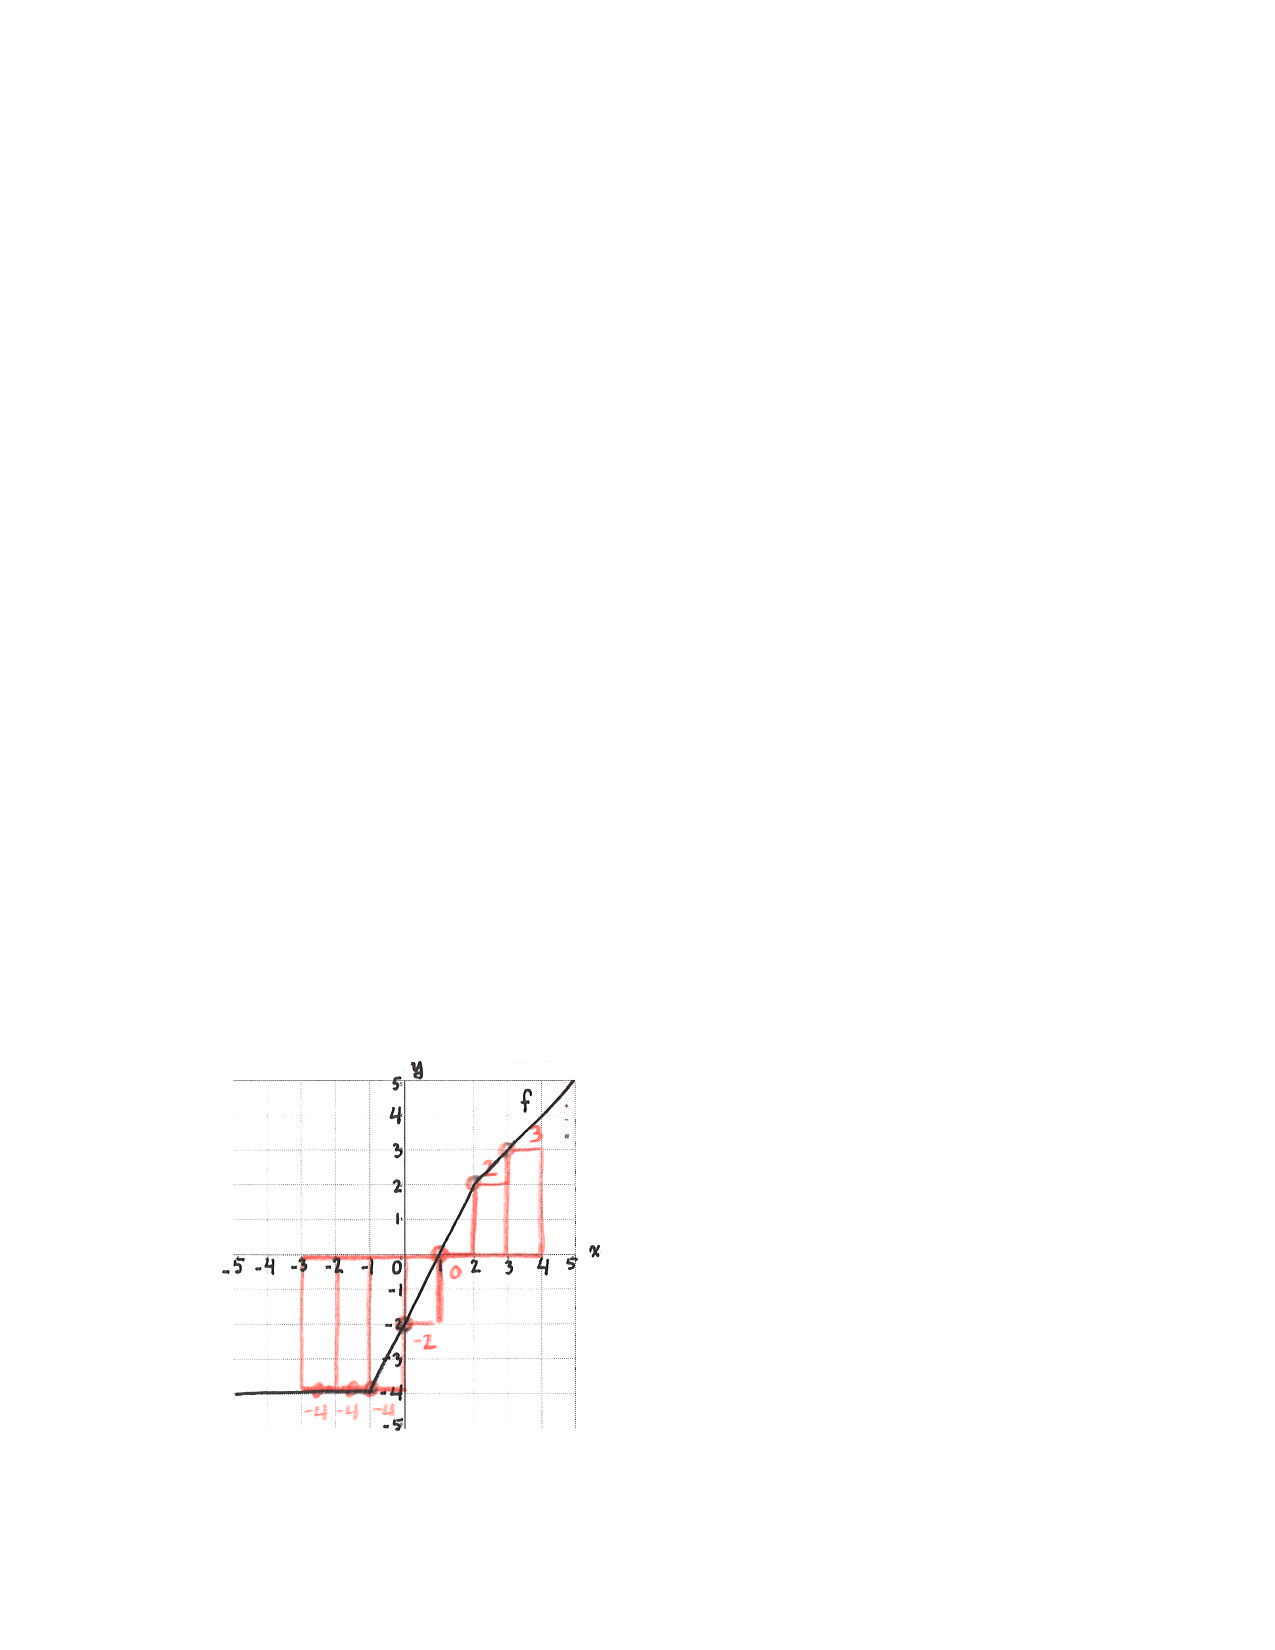
\includegraphics[scale=0.8]{\filePathGraphics/LQ13_Graph_Lower.pdf}% Activate for solutions.
\hspace{1in}
%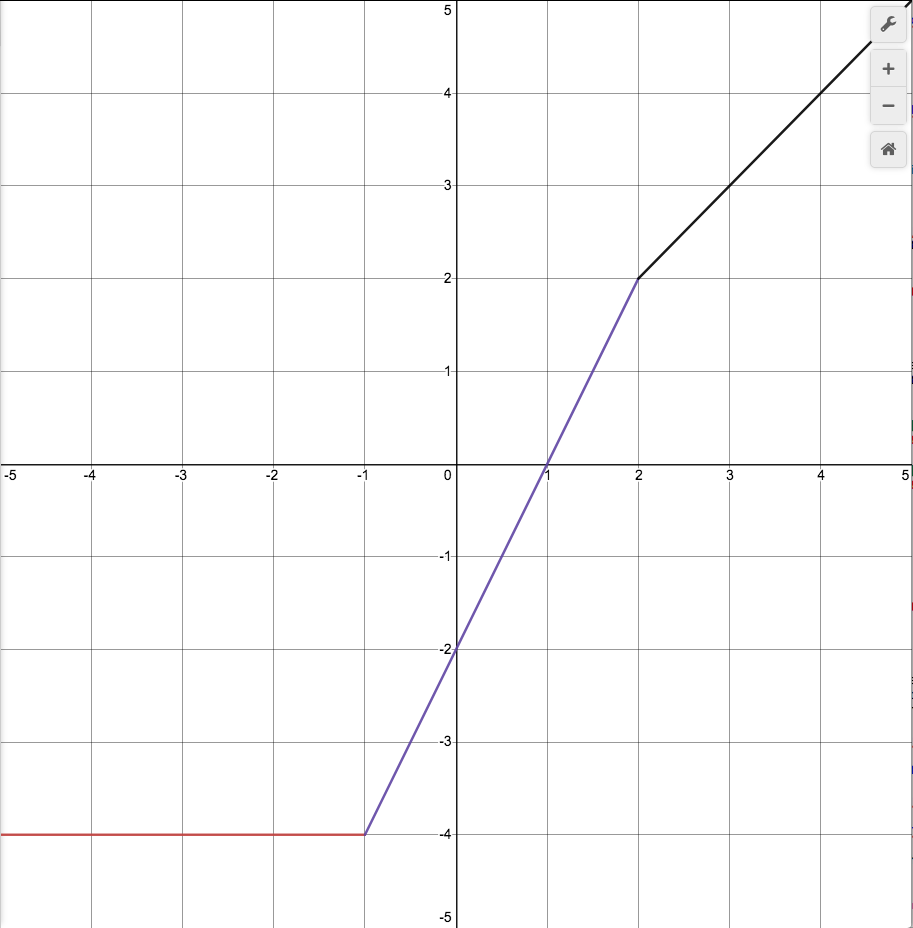
\includegraphics[scale=0.18]{\filePathGraphics/LQ13_Graph.png}% Activate for quiz.
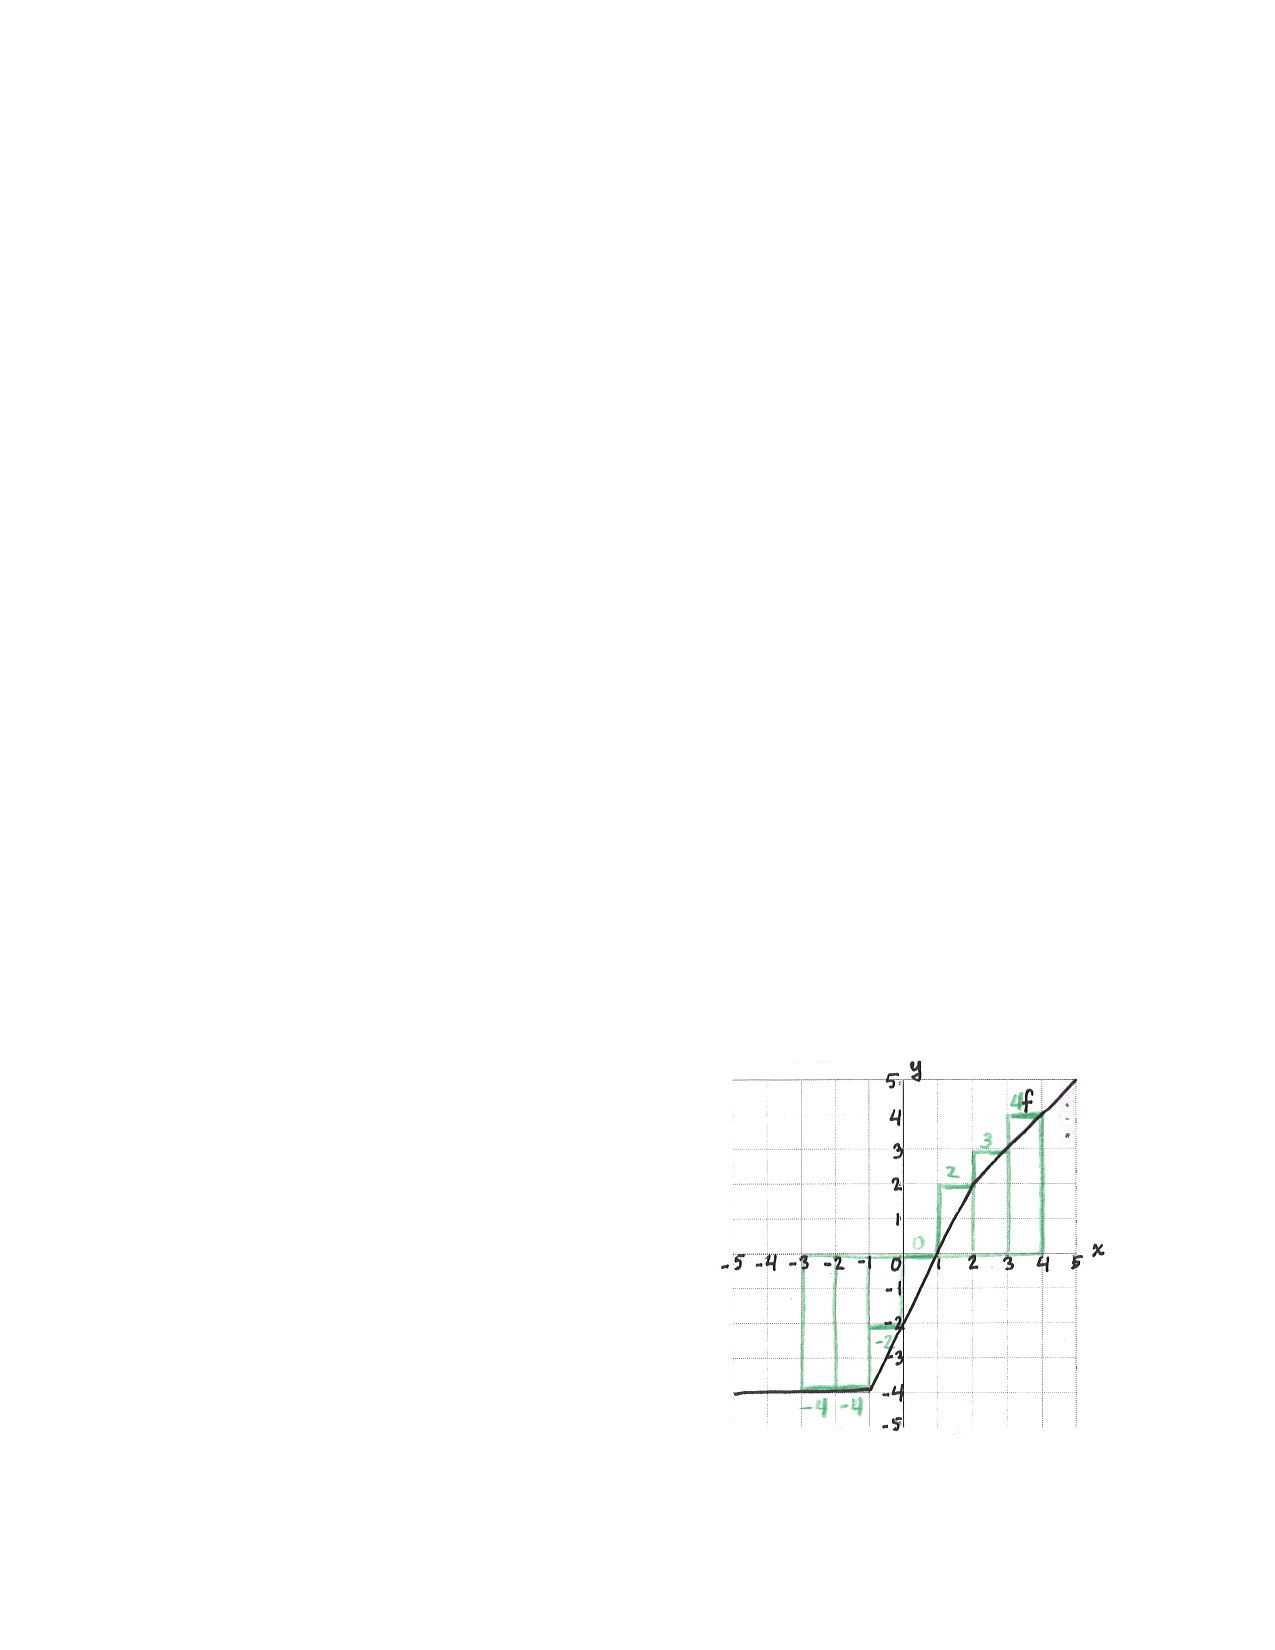
\includegraphics[scale=0.8]{\filePathGraphics/LQ13_Graph_Upper.pdf}% Activate for solutions.
\\
Lower sum ($L$)
\hspace{2.3in}
Upper sum ($U$)
\end{center}
\end{enumerate}

\spaceSolution{1in}{% Begin solution.
The lower sum $L$ and upper sum $U$ are sketched above. We compute the value of each by adding the (signed) areas of their rectangles:
\begin{align*}
L
&=
-4 + (-4) + (-4) + (-2) + 0 + 2 + 3
=
-9
\\
U
&=
-4 + (-4) + (-2) + 0 + 2 + 3 + 4
=
-1
\end{align*}
Using our result from part \ref{itm : LQ13a}, we confirm that
\begin{align*}
L
&=
-9
&
\leq
&&
\int_{-3}^{4} f(x) \spaceIntd \intd x
&=
-5
&
\leq
&&
U
&=
-1
\end{align*}}% End solution.



\noindent{}For reference, $f : \reals \rightarrow \reals$ is the piecewise function whose rule of assignment is
\begin{align*}
f(x)
=
\begin{dcases*}
-4		&	if $x \leq -1$		\\
2 x - 2	&	if $-1 \leq x \leq 2$	\\
x		&	if $x \geq 2$
\end{dcases*}
\end{align*}

\begin{enumerate}[resume,label=(\alph*)]
\item\label{itm : LQ13c} (1 pt) Find an antiderivative $F_{i}(x)$ for each ``piece'' of $f(x)$. Use these antiderivatives and the fundamental theorem of calculus to compute the value of each integral on the right side of the following equation:
\begin{align}
\int_{-3}^{4} f(x) \spaceIntd \intd x
=
\int_{-3}^{-1} f(x) \spaceIntd \intd x
+
\int_{-1}^{2} f(x) \spaceIntd \intd x
+
\int_{2}^{4} f(x) \spaceIntd \intd x%
\label{eq : LQ13 Piecewise Integral}
\end{align}
Add your values for the three integrals on the right, and compare the result to part \ref{itm : LQ13a}.
\end{enumerate}

\spaceSolution{3in}{% Begin solution.
Let $f_{i}(x)$ denote the rule of assignment for each ``piece'' of $f(x)$. That is,
\begin{align*}
f_{1}(x)
&=
-4
&
f_{2}(x)
&=
2 x - 2
&
f_{3}(x)
&=
x
\end{align*}
We compute an antiderivative for each of these functions (on their respective intervals):
\begin{align*}
F_{1}(x)
&=
-4 x
&
F_{2}(x)
&=
x^{2} - 2 x
&
F_{3}(x)
&=
\frac{1}{2} x^{2}
\end{align*}
Using these, and the fundamental theorem of calculus, we compute the value of each integral on the right side of Equation \eqref{eq : LQ13 Piecewise Integral}:
\begin{align*}
\int_{-3}^{-1} f(x) \spaceIntd \intd x
&=
F_{1}(-1) - F_{1}(-3)
=
\left[(-4)(-1)\right] - \left[(-4)(-3)\right]
=
4 - 12
=
-8
\\
\int_{-1}^{2} f(x) \spaceIntd \intd x
&=
F_{2}(2) - F_{2}(-1)
=
\left[(2)^{2} - 2 (2)\right] - \left[(-1)^{2} - 2 (-1)\right]
=
0 - 3
=
-3
\\
\int_{2}^{4} f(x) \spaceIntd \intd x
&=
F_{3}(4) - F_{3}(2)
=
\left[\frac{1}{2} (4)^{2}\right] - \left[\frac{1}{2} (2)^{2}\right]
=
8 - 2
=
6
\end{align*}
Referring to Equation \eqref{eq : LQ13 Piecewise Integral}, adding these three results gives
\begin{align*}
\int_{-3}^{4} f(x) \spaceIntd \intd x
=
(-8) + (-3) + 6
=
-5
\end{align*}
This equals the exact value of the definite integral that we computed in part \ref{itm : LQ13a}, as the fundamental theorem of calculus guarantees.}% End solution.